 \documentclass{article}

\usepackage{mystyle}

\setenumerate[0]{label=(\alph*)} % Set default of enumerate to be alphabetical
\graphicspath{ {./img/} } % path to image folder

\begin{document}

\maketitle

\newpage

\tableofcontents

\newpage

\section{Problem A: Cart-pole}

\paragraph{Note on value function representation}

For all of the value functions we have used the form where we take as input the
current state $s_t$ which then maps through $Q$ to the action space, giving a
score to each possible action. For the cart pole we have that $a_t \in \{0, 1\}
= A$ and $s_t \in \{([-2.4, 2.4], \mathbb{R}, [-41.8, 41.8], \mathbb{R})\} = S$,
which represents cart position, cart velocity, pole angle and pole velocity at tip.
This means that we have a value function $Q: S \to A$. In order to find the
action-value for the pair $(s_t, a_t)$ we just look at index $a_t$ of $Q(s_t)$
such that $Q(s_t, a_t) := [Q(s_t)]_{a_t}$.

\paragraph{How statistics was collected}

All of the statistics was collected by bringing the agent out of the training
regime and evaluated on the environment using the learned greedy policy on 20
episodes normally, although this differs slightly depending on how
computationally demanding the task was and what was asked for in the question.

I saved the models every time I saw an improvement in test performance while
running training, which is why most of them get close to 300 episode length when
evaluated.

\paragraph{Hyperparameters}

For each of the questions we used similar hyperparameters. For optimization we
used ADAM since it worked better than SGD and similar or better than RMSprop
even though RMSprop is said to be suitable for RL problems. The networks did not
use extra implementations such as regularisation and/or batch normalisation
since this didn't seem necessary.

I used the following learning rate, batch size, buffer size and epochs for each
subquestion.

\begin{center}
  \makebox[\textwidth][c]{
    \begin{tabular}{|c|c|c|c|c|c|c|c|} 
      \hline
      Question & optimizer & decay schedule & learning rate & batch size & buffer size & epochs/episodes & Hidden units \\
      \hline
      A3 & ADAM & None & Various & 16 & - & 500 & - \\
      \hline
      A4 & ADAM & None & 0.0001 & - & - & 2000 & 100 \\
      \hline
      A5 & ADAM & None & 0.0001 & - & - & 2000 & 30/1000 \\
      \hline
      A6 & ADAM & Polynomial & 0.0001 & 32 & 10000 & 2000 & 100 \\
      \hline
      A7 & ADAM & None & 0.0001 & 32 & 10000 & 2000 & 100 \\
      \hline
    \end{tabular}
  }
\end{center}

For the polynomial decay I used the builtin Tensorflow
\texttt{tf.train.polynomial\_decay} such that the learning rate that you choose
is the starting learning rate, the end learning rate was set to be 0.000001,
decay steps 100000 and power to 0.5.

\subsection{Generate three trajectories under a uniform random policy. Report
  the episode lengths and the return from the initial state.}

We have the following episode lengths and total discounted returns from the
initial state under a uniformly random policy:

\begin{center}
  \begin{tabular}{ |c|c|c|c| } 
    \hline
    Run  & 1 & 2 & 3 \\
    \hline
    Episode length & 20 & 19 & 16 \\ 
    Total discounted reward & -0.8179 & -0.8262 & -0.8515 \\
    \hline
  \end{tabular}
\end{center}

\subsection{Generate 100 episodes under the above random policy, and report the
  mean and standard deviation of the episode lengths and the return from the
  starting state.}

We get the following figures:

\begin{center}
  \begin{tabular}{ |c|c|c| }
    \hline
     & mean & std. \\
    \hline
    Episode length & 22.53 & 11.717 \\ 
    Total discounted reward & -0.8027 & 0.0898 \\
    \hline
  \end{tabular}
\end{center}

\subsection{Collect 2000 episodes under a uniformly random policy and implement
  batch Q-learning to learn to control the cart-pole.}

We first sample 2000 episodes worth of tuples of $(S_t, A_t, R_{t+1}, S_{t+1})$,
through a uniformly random policy. After gathering about $44000$ such tuples, as
the mean length of an episode is about 22, we
train agents running offline batch Q-learning to learn the optimal policy
of controlling the cart-pole. For this part we consider 5 different learning
rates, $[10^{-5}, 10^{-4}, 10^{-3}, 10^{-2}, 10^{-1}, 0.5]$ and two different
value function approximators:

\begin{description}
\item[Linear]
  \begin{equation*}
    Q(S_t, A_t) = [S_t^TW + b]_{A_t}
  \end{equation*}

  Since $|A| = 2$ and $|S| = 4$ we have that if we represent vectors in column
  form that $W \in \mathbb{R}^{4 \times 2}, b \in \mathbb{R}^{1 \times 2}$.
\item[MLP]
  For the Multi-Layer Perceptron we have that
  \begin{equation*}
    Q(S_t, A_t) = [\sigma(S_t^TW_1 + b_1)W_2 + b_2]_{A_t}
  \end{equation*}

  Were we have the freedom to choose the hidden layers $H$ such that $W_1 \in
  \mathbb{R}^{4 \times H}, b \in \mathbb{R}^{H}, W_2 \in \mathbb{R}^{H \times 2},
  b_2 \in \mathbb{R}^{2}$, and $\sigma$ represents an elementwise sigmoid
  function, in our case the ReLU. This is true for all the different networks
  below as well, with different $H$ depending on the subquestion. In this case
  $H = 100$.
\end{description}

\subsubsection{Linear}

We have the following plots

\begin{figure}[H]
  \centering
  \begin{minipage}{0.45\textwidth}
    \centering
    \includegraphics[width=0.9\textwidth]{A3/{A3linear0.5}.png}
    \caption{Learning rate: 0.5}
  \end{minipage}\hfill
  \begin{minipage}{0.45\textwidth}
    \centering
    \includegraphics[width=0.9\textwidth]{A3/{A3linear0.1}.png}
    \caption{Learning rate: 0.1}
  \end{minipage}
\end{figure}

\begin{figure}[H]
  \centering
  \begin{minipage}{0.45\textwidth}
    \centering
    \includegraphics[width=0.9\textwidth]{A3/{A3linear0.01}.png}
    \caption{Learning rate: 0.01}
  \end{minipage}\hfill
  \begin{minipage}{0.45\textwidth}
    \centering
    \includegraphics[width=0.9\textwidth]{A3/{A3linear0.001}.png}
    \caption{Learning rate: 0.001}
  \end{minipage}
\end{figure}

\begin{figure}[H]
  \centering
  \begin{minipage}{0.45\textwidth}
    \centering
    \includegraphics[width=0.9\textwidth]{A3/{A3linear0.0001}.png}
    \caption{Learning rate: 0.0001}
  \end{minipage}\hfill
  \begin{minipage}{0.45\textwidth}
    \centering
    \includegraphics[width=0.9\textwidth]{A3/{A3linear0.00001}.png}
    \caption{Learning rate: 0.00001}
  \end{minipage}
\end{figure}

\subsubsection{100-hidden units MLP}

We have the following plots

\begin{figure}[H]
  \centering
  \begin{minipage}{0.45\textwidth}
    \centering
    \includegraphics[width=0.9\textwidth]{A3/{A3NNet0.5}.png}
    \caption{Learning rate: 0.5}
  \end{minipage}\hfill
  \begin{minipage}{0.45\textwidth}
    \centering
    \includegraphics[width=0.9\textwidth]{A3/{A3NNet0.1}.png}
    \caption{Learning rate: 0.1}
  \end{minipage}
\end{figure}

\begin{figure}[H]
  \centering
  \begin{minipage}{0.45\textwidth}
    \centering
    \includegraphics[width=0.9\textwidth]{A3/{A3NNet0.01}.png}
    \caption{Learning rate: 0.01}
  \end{minipage}\hfill
  \begin{minipage}{0.45\textwidth}
    \centering
    \includegraphics[width=0.9\textwidth]{A3/{A3NNet0.001}.png}
    \caption{Learning rate: 0.001}
  \end{minipage}
\end{figure}

\begin{figure}[H]
  \centering
  \begin{minipage}{0.45\textwidth}
    \centering
    \includegraphics[width=0.9\textwidth]{A3/{A3NNet0.0001}.png}
    \caption{Learning rate: 0.0001}
  \end{minipage}\hfill
  \begin{minipage}{0.45\textwidth}
    \centering
    \includegraphics[width=0.9\textwidth]{A3/{A3NNet0.00001}.png}
    \caption{Learning rate: 0.00001}
  \end{minipage}
\end{figure}

From all this we see that the linear learner does a pretty good job at solving
the Cartpole problem, getting to 300 and hovering there for a learning rate of
0.001. However, for other values we have more erratic behaviour and given the
volatile nature of RL, it might have been pure luck since other runs for lower
learning rates give less stable runs as can be seen in the figures for learning
rate 0.0001 and 0.00001.

While the neural net is more powerful than the linear learner as it can
represent a bigger space of functions, it is also more volatile and prone to
catastrophic forgetting. An interesting phenomenon is that in many of these runs
the neural networks learn a decent policy (such as in the figure of learning
rate 0.0001) even though the bellman loss seems to converge. An example of
destructive learning can be found in the figure of the learning rate 0.00001.

\subsection{Function approximation using Q-learning.}

We implement an online Q-learning algorithm using an MLP for function
approximation as specified above. We let the hidden layer be of size 100 and
non-linearity being the ReLU function outputting a value for each possible
action 0 and 1.

Using this we have that the bellman residual is

\begin{equation*}
  \delta = R_{t+1} + \gamma \max_{a} Q(S_{t + 1}, a) - Q(S_t, A_t)
\end{equation*}

and the loss

\begin{equation*}
  Loss = 0.5 \delta^2.
\end{equation*}

We train the agent using an epsilon greedy policy with $\epsilon = 0.05$ over
$2000$ episodes. To evaluate performance we let the agent run 20 episodes using
a greedy policy with regards to the current $Q_t$ at the finished training
episode. During evaluation we don't train. We then take the mean of the episode
length, total discounted reward and Bellman loss over these 20 evaluation
episodes and the let the means be representative of the agent at that point in
time.

We plot all of the learning traces using a small alpha for the opacity and the
line specifies the mean of the 100 traces.

\begin{figure}[H]
  \centering
  \includegraphics[width=0.9\textwidth]{A4/{A40.001}.png}
  \caption{Learning traces}
\end{figure}

From the plot we see the inherent volatility and variance using the same
algorithm (Q-learning) on the same environment (CartPole-v0) with identical
hyperparameters. From the traces we see that at most episodes during training we
have traces which have an average episode length of 9 to 300, echoing the fact
that their will be agents that oscillate between optimal (300) and worst case
(9) scenario. However, on average we have decent behaviour of around 200.
However, since we cap the maximal episode length at 300, we have that the mean
will always be below 300 and thus be biased towards a lower value of episode
lengths than if we actually evaluated the episode length of an unconstrained
environment.

If we look at the Bellman residue we can see that this shows that we almost
always overestimate our current Q-action-value function compared to the target,
as found in the Double Q-learning paper\footnote{https://arxiv.org/pdf/1509.06461.pdf}.

\subsection{Network with ReLUs and different hidden units.}

We reuse the same network as in the previous question but with different number
of hidden units, $30$ and $1000$.

\begin{figure}[H]
  \centering
  \includegraphics[width=0.9\textwidth]{A5/{A5a0.0001}.png}
  \caption{30 hidden units}
\end{figure}

\begin{figure}[H]
  \centering
  \includegraphics[width=0.9\textwidth]{A5/{A5b0.00001}.png}
  \caption{1000 hidden units}
\end{figure}

From the graphs we see the volatility of online Q-learning. I found while
training that the 30-unit networks converged quicker than the 1000 unit
networks, which makes sense since the smaller network should be faster to
converge. In both cases, by running and testing for optimal hyperparamters, I
experienced that the networks where prone to catastrophic  
forgetting where they would learn a policy which reach 300 average episode
length (Since the evaluation was over 20 episodes, this also means that it must
have gotten a length of 300 for all episodes since we take the mean.)
essentially solving the problem, only to forget everything later and getting a
policy that consistently gave an average episode length of about 9.5.

The difference between the 30 and the 1000 unit network was not as big as I
would have thought. However, our problem here consists of finding the optimal
network over an online period of 2000 episodes. This means that we are not
really finding the network that learns the best policy overall, but the best
policy over 2000 episodes (which is a pretty big constraint as we normally train
over epochs of data sets of size 2000 and more). I imagine that training over a
longer period of episodes and a lower learning rate would mean that the more
flexible 1000 hidden unit network would learn a better policy and potentially
mitigate the catastrophic forgetting.

\subsection{Experience replay.}

We reuse the same network as in previous questions but add an experience replay
buffer where we store the previous tuples up to a certain point, which is
specified by the buffer size. This should stabilise the learning since we can
both batch and reuse previous experience to learn.

We have the following graph

\begin{figure}[H]
  \centering
  \includegraphics[width=0.9\textwidth]{A6/{A6}.png}
  \caption{100 hidden units}
\end{figure}

Compared to the previous question we see that the experience replay buffer has a
stabilising effect on the bellman residual, meaning that we converge to a policy
that is consistent much quicker. We also note that the overestimation of the
Q-value seem to have disappeared since the Bellman residual is now distributed
more evenly around zero and not consistently negative as before.

The experience replay buffer makes sure that we can both batch while training,
meaning we may learn faster as we take more aspects of the data into
consideration as we run backpropagation, stabilise the backpropagation and also
decouples the data points making batches for sequential training steps less
correlated, while improving data efficiency\footnote{p.7, https://storage.googleapis.com/deepmind-media/dqn/DQNNaturePaper.pdf}.

While the bellman residue and thus the loss is improved the most, it also
mitigates the volatility of the performance of the network. While it still have
catastrophic forgetting, it doesn't seem to be as volatile as in previous
questions. However, as we are only doing one run, it's hard to tell properly.

\subsection{Compare using a target network}

Similarly to above we have a experience replay buffer but also add a target
network. Using a target network means that we should stabilise learning as we
decouple the update with the current network, removing possible feedback loops
due to the target being dependent on the network at the current timestep. By
only copying the network at certain intervals we break this dependency since the
correlation dies out quickly as we progress in time.

We have the following graph

\begin{figure}[H]
  \centering
  \includegraphics[width=0.9\textwidth]{A7/{A7}.png}
  \caption{100 hidden units}
\end{figure}

It's hard to tell if a target network actually improve things. I think that over
time the target network should be able to use the data more efficiently rather
than over the period of just 2000 episodes.

What is clear though is that the target network reduces the bias of the Q-value
function. Looking at the residual graph we see that it is much more evenly
distributed around 0 and not predominantly on one side of the origin (i.e
negative as before, due to Q-learning being biased.).

From this we can clearly see the theoretical advantage of a target network. It
decouples the target Q-value from the current policy and thus makes the data
less biased towards our current policy, leading to data that is less correlated
and should be easier to train on.

\subsection{Compare Sarsa to previous performance}

Not implemented.

\newpage

\section{Problem B: Atari games}

\subsection{Report the score and frame counts from the three games under a
  random policy, evaluated on 100 episodes. Report both the average and the
  standard deviation.}

We have the following table

\begin{center}
  \begin{tabular}{ |c|c|c|c|c| } 
    \hline
    Game & score (mean) & score (std) & frame count (mean) & frame count (std) \\
    \hline
    Pong & -0.9059 & 0.2707 & 1225.86 & 137.19 \\
    \hline
    Ms. Pacman & 2.4412 & 0.5758 & 636.03 & 100.74 \\
    \hline
    Boxing & -0.4100 & 1.1064 & 2378.26 & 13.87 \\
    \hline
  \end{tabular}
\end{center}

\subsection{Report performance on the three games from an initialized but
  untrained Q-network, evaluated on 100 episodes. Explain why the performance
  can be different from part one.}

We have the following table

\begin{center}
  \begin{tabular}{ |c|c|c|c|c| } 
    \hline
    Game & score (mean) & score (std) & frame count (mean) & frame count (std) \\
    \hline
    Pong & -1.1302 & 0.0317 & 1018.65 & 8.96 \\
    \hline
    Ms. Pacman & 2.8629 & 0.1980 & 578.83 & 134.55 \\
    \hline
    Boxing & -3.3297 & 1.4200 & 1429.05 & 263.3219 \\
    \hline
  \end{tabular}
\end{center}

The statistics differ from that of the uniform policy simply since a CNN which
is randomly initialized will probably be biased towards different actions even
though it is not trained. For example filters which are randomly initilized will
often still be able to find some natural shapes (Similar to Gabor filters) and
thus act in some manner which is non-random, although suboptimal.

\subsection{Plot the losses of your agent during the course of training. Discuss
  the shapes of the curves and why they might differ from supervised learning.}

We have the following plots

\subsubsection{Pong}

\begin{figure}[H]
  \centering
  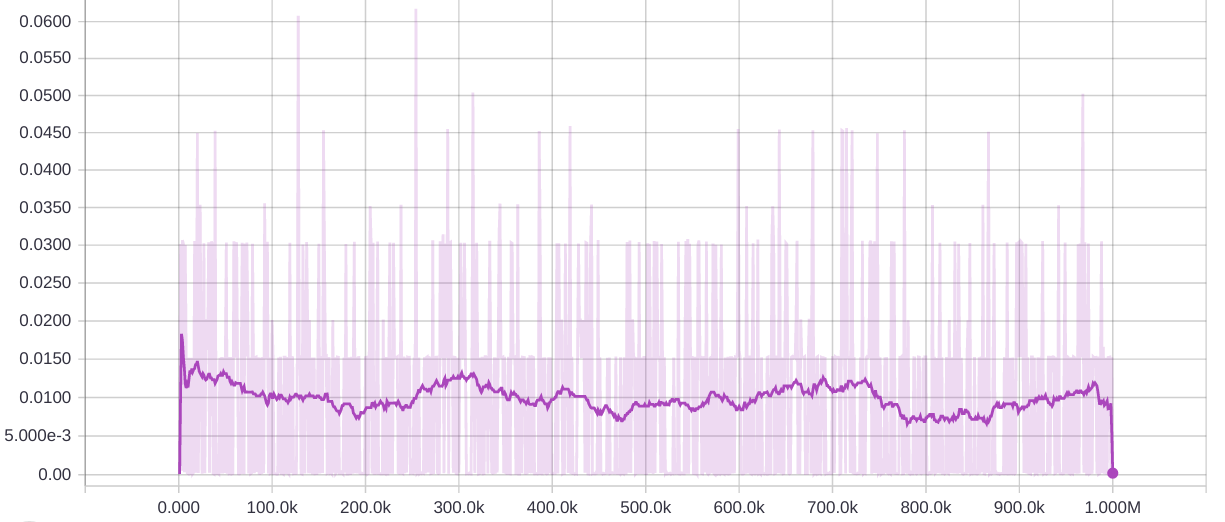
\includegraphics[width=0.9\textwidth]{B3/pong_loss.png}
  \caption{Loss}
\end{figure}

\begin{figure}[H]
  \centering
  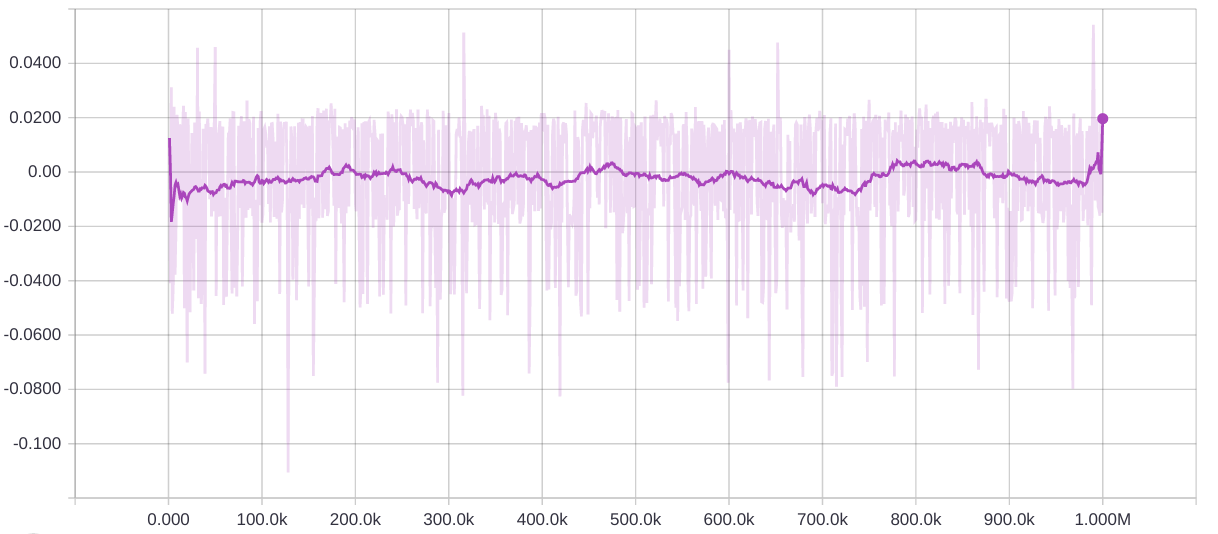
\includegraphics[width=0.9\textwidth]{B3/pong_residual.png}
  \caption{Residual}
\end{figure}

\subsubsection{Ms Pacman}

\begin{figure}[H]
  \centering
  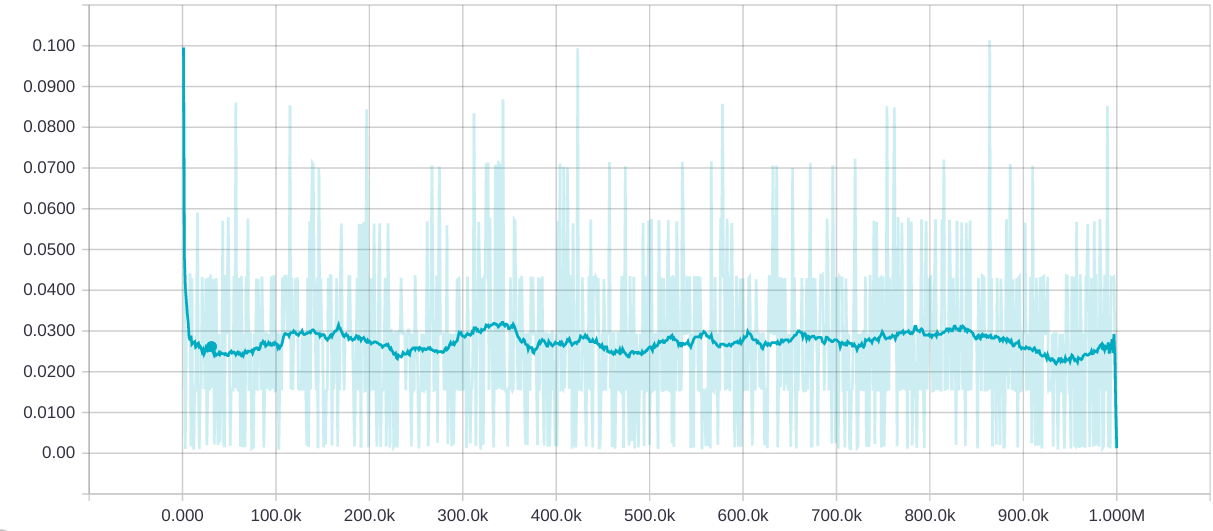
\includegraphics[width=0.9\textwidth]{B3/pacman_loss.png}
  \caption{Loss}
\end{figure}

\begin{figure}[H]
  \centering
  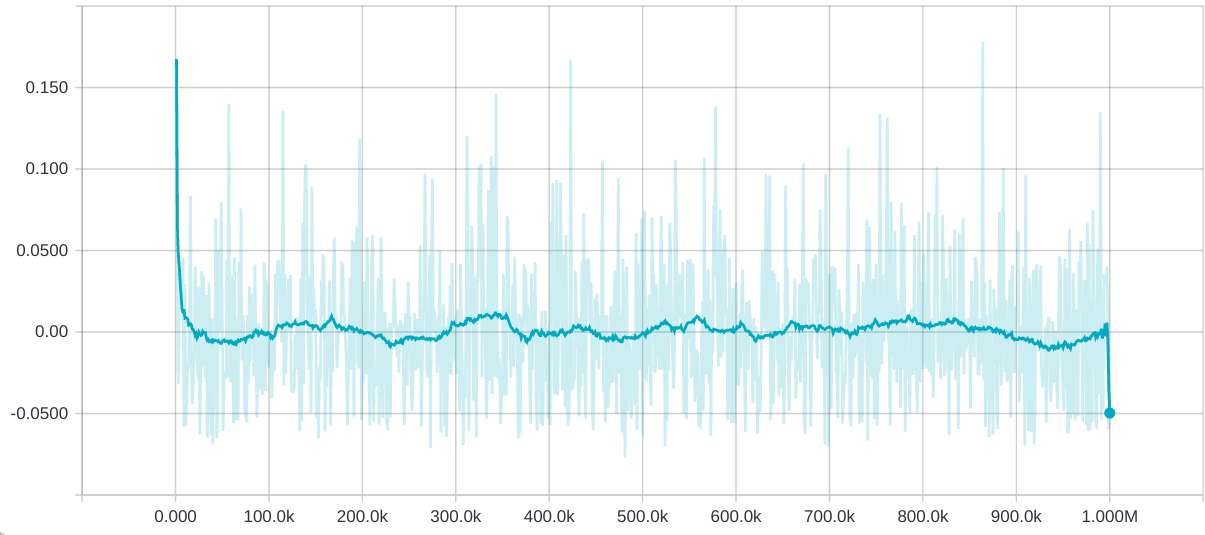
\includegraphics[width=0.9\textwidth]{B3/pacman_residual.png}
  \caption{Residual}
\end{figure}

\subsubsection{Boxing}

\begin{figure}[H]
  \centering
  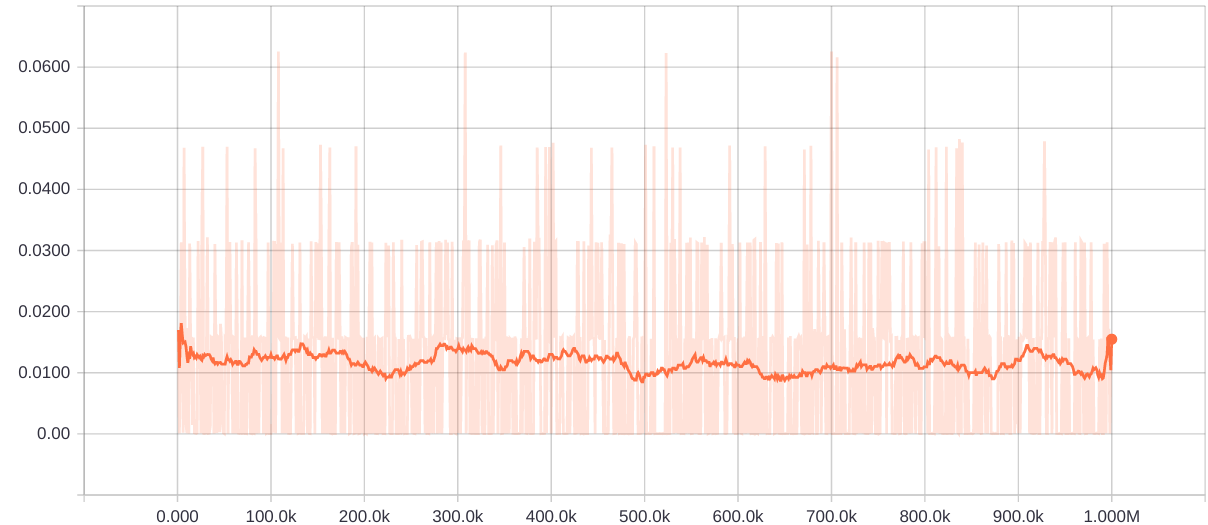
\includegraphics[width=0.9\textwidth]{B3/boxing_loss.png}
  \caption{Loss}
\end{figure}

\begin{figure}[H]
  \centering
  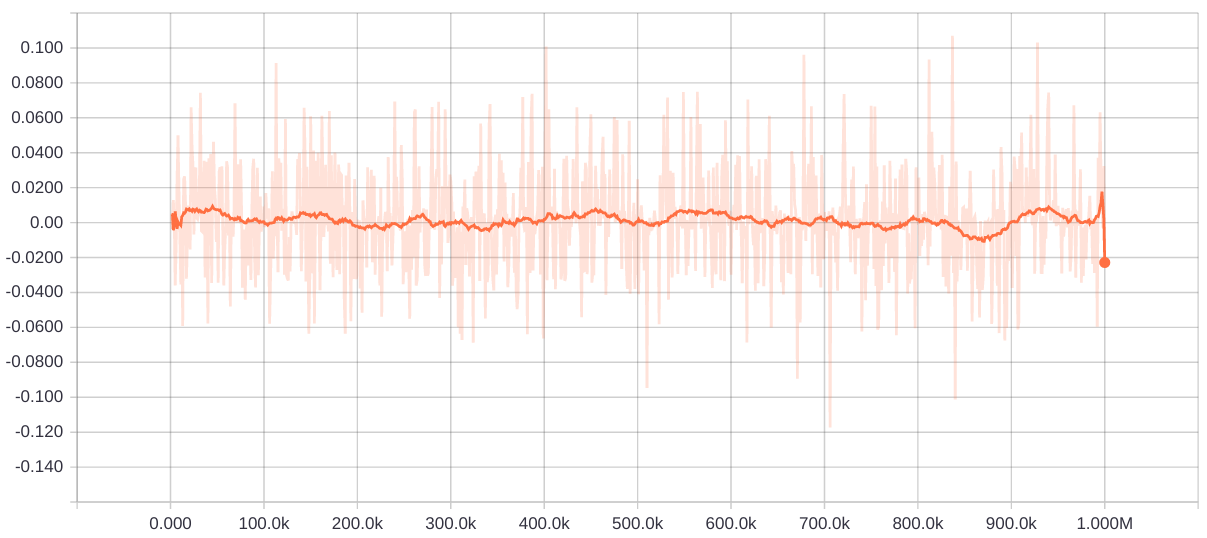
\includegraphics[width=0.9\textwidth]{B3/boxing_residual.png}
  \caption{Residual}
\end{figure}

We see that the plots of the losses have a slow decrease, although these plots
are a running average of the loss and thus smoother than they actually are raw.
From A we know that the loss is not completely representative of the actual
performance of the agent, as we might find a policy which has low loss, but
actually is stuck in a bad state, not getting a very good performance (which
might be different from the actual discounted reward which relates directly to
our loss).

If we were to compare these loss curves to those of Supervised Learning, the
difference would have to do with the fact that in RL we are able to interact
with the environment, affecting the future states through our actions. In SL we
don't do this, instead we simply try to predict the outcome given the input, but
we can't change the behaviour of the environment from this. Specifically, in SL
we assume that the data is i.i.d while in RL we don't have any such guarantees
since the distribution of the states depends on the policy which itself changes
with time.

\subsection{Report the final performance in terms of cumulative undiscounted
  rewards per episode of your trained agent, averaged over 100 episodes.
  Describe any modifications to the above by which you were able to improve
  performance in this limited data regime.}

We have the following table for the averaged cumulative undiscounted rewards per
episode of the trained agents.

\begin{center}
  \begin{tabular}{ |c|c|c|c| } 
    \hline
     & Pong & MsPacman & Boxing \\
    \hline
    Cumulative undiscounted reward & -21.0 & 21.0 & -2.27 \\
    \hline
  \end{tabular}
\end{center}

As can be seen this is not very good and for the games Pong and MsPacman I
consistently get these scores, 21 and -21. Boxing differs from episode and have
a higher variability. The reason why my agent fails to learn is twofold.

Since we downsize the frames to 28x28, we almost lose all of the visual cues
needed to play the game. There is still enough information to actually learn a
policy, but learning it is non-trivial and not easy. I think what happens is
that the agent start off gaining some score, as in pacman, and continue this
policy indefinitely. Still, the loss function changes so some kind of learning
or at least adjustment of the policy through time occurs.

As we only train for a million steps, this might actually be too little to be
able to learn a non-trivial policy. We use both experience replay and target
network so this in some way decouples the data and should enable the agent to
learn in a more stable manner than without it, but the number of iterations
might not be enough to actually establish a policy different from the starting
one.

I didn't have time to experiment with hyperparameters but given the time I would
try different ways of downsampling that would leave more of the image intact,
such as clipping it in an intelligent way such that the 28x28 is a patch rather
than a downsized version of the original image. I would also look into using
more complex learning rate schemes and see if a higher epsilon for exploring would
improve the policy as more of the states would be investigated than is now.

\appendix

\end{document}
